
\begin{center}
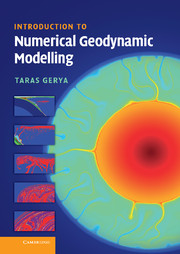
\includegraphics[height=4.5cm]{images/literature/gerya_book}
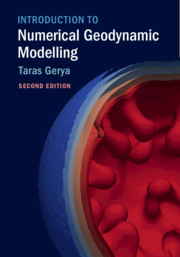
\includegraphics[height=4.5cm]{images/literature/gerya_book2}
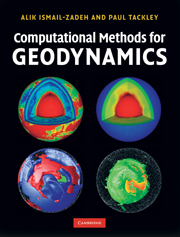
\includegraphics[height=4.5cm]{images/literature/tackley_book}
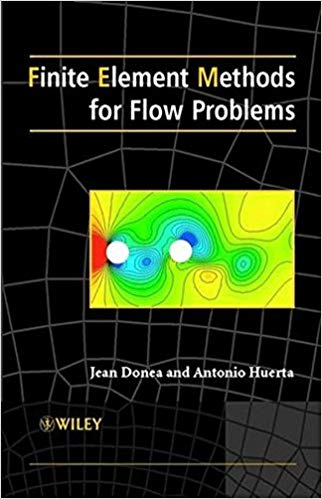
\includegraphics[height=4.5cm]{images/literature/donea_huerta_book}\\
\cite{gery10} \hspace{1.99cm} 
\cite{gery19book} \hspace{1.99cm} 
\cite{tack10} \hspace{1.99cm} 
\cite{dohu03}  \\
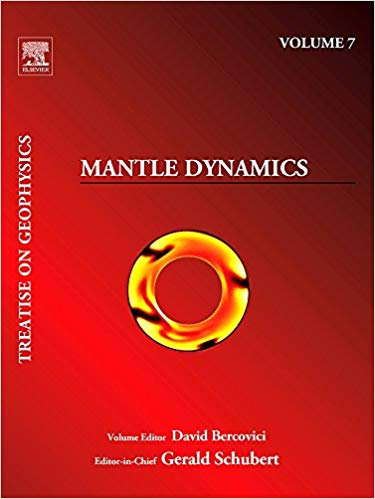
\includegraphics[height=4.5cm]{images/literature/bercovici_book}
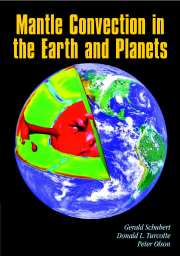
\includegraphics[height=4.5cm]{images/literature/sto_book}
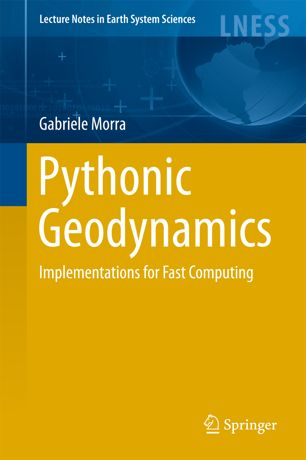
\includegraphics[height=4.5cm]{images/literature/morra_book}
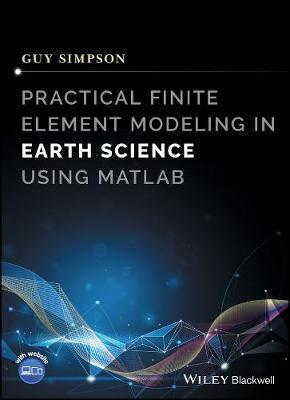
\includegraphics[height=4.5cm]{images/literature/simpson_book}\\
\cite{berc09} \hspace{1.99cm} 
\cite{scto01} \hspace{1.99cm} 
\cite{morr18} \hspace{1.99cm} 
\cite{simp17}
\end{center}

\begin{itemize}
\item {\it Numerical modeling of Earth Systems} by Thorsten W. Becker and Boris J. P. Kaus,\\ 
\url{http://www-udc.ig.utexas.edu/external/becker/teaching-557.html}

\item {\it Myths \& Methods in Modeling} by M. Spiegelman,\\
 \url{https://www.ldeo.columbia.edu/~mspieg/mmm/}

\item {\it Computational Science I} by Matthew G. Knepley,\\
 \url{https://cse.buffalo.edu/~knepley/classes/caam519/Syllabus.html}

\item {\it Introduction to Numerical Methods for Variational Problems} by Hans Petter Langtangen and 
Kent-Andre Mardal, \\
\url{https://hplgit.github.io/fem-book/doc/pub/book/pdf/fem-book-4print.pdf}
\end{itemize}

